\documentclass[11pt,a4paper]{article}
\usepackage[margin=2.1cm]{geometry}
\usepackage{fontspec,amsmath,amssymb,graphicx,booktabs,tabularx,array,caption,float,xcolor}
\setmainfont{Noto Serif}
\setsansfont{Noto Sans}
\definecolor{navy}{HTML}{244B68}
\usepackage[colorlinks=true,linkcolor=navy]{hyperref}
\usepackage{titlesec}
\titleformat{\section}{\large\bfseries\color{navy}}{\Roman{section}.}{.6em}{}
\titleformat{\subsection}{\normalsize\bfseries}{\Alph{subsection}.}{.6em}{}
\setlength{\parindent}{1em}\setlength{\parskip}{4pt}
\captionsetup{font=small,labelfont=bf}
\renewcommand{\figurename}{Hình}\renewcommand{\tablename}{Bảng}
\newcommand{\fig}[3]{\begin{figure}[H]\centering\includegraphics[width=#2\linewidth]{figures/#1.pdf}\caption{#3}\end{figure}}
\begin{document}
\begin{center}
{\small\sffamily BÁO CÁO BÀI TẬP LỚN GIỮA KỲ • TRÍ TUỆ NHÂN TẠO 2026–2027}\par\medskip
{\LARGE\bfseries Tìm kiếm đối kháng và tìm kiếm cây Monte Carlo với UCT}\par\medskip
{\large Cơ sở lý thuyết, các biến thể công thức và ứng dụng trong Tic-Tac-Toe, Caro, Cờ tướng và lập lịch giao hàng}\par\medskip
{\small Bản dịch tiếng Việt — Tác giả sinh viên}
\end{center}
\noindent\textbf{Tóm tắt—} Bài báo triển khai, phân tích và đánh giá thực nghiệm Minimax kết hợp cắt tỉa Alpha–Beta và tìm kiếm cây Monte Carlo sử dụng cận tin cậy trên áp dụng cho cây (MCTS–UCT) trên Tic-Tac-Toe 3×3, Caro 5 quân liên tiếp, Cờ tướng 9×10 và bài toán định tuyến giao hàng chặng cuối có ràng buộc khung thời gian (TSP-TW). Nghiên cứu xây dựng UCT từ bất đẳng thức Hoeffding và lý thuyết Multi-Armed Bandit, giải thích phép căn bậc hai và logarithm, đồng thời đánh giá bảy biến thể UCT (bao gồm UCB1-Tuned và PUCT dùng thông tin tiên nghiệm heuristic) cùng các phương pháp mô phỏng ngẫu nhiên, heuristic chiến thuật và Value-Cutoff. Kết quả cho thấy Alpha–Beta có sắp xếp nước đi giảm số nút duyệt 98,57\% trên Tic-Tac-Toe 3×3 (99,61\% với bảng chuyển vị), 93,29\% trên Caro 9×9 và 93,44\% trên Cờ tướng, vẫn giữ nguyên giá trị Minimax chính xác. Trên Tic-Tac-Toe, MCTS–UCT đạt tỷ lệ thua 0\% trong 100 ván luân phiên với Alpha–Beta tối ưu từ 500 vòng lặp. Trên Caro, Value-Cutoff nâng tỷ lệ thắng từ 16\% (ngẫu nhiên) và 34\% (heuristic) lên 74\%, nhanh hơn 6,2 lần so với mô phỏng heuristic đầy đủ; PUCT đạt 98\%. Với TSP-TW, MCTS heuristic đạt độ sai lệch tối ưu 4,78\% so với nhánh cận chính xác và giảm chi phí 43,6\% so với tham lam chọn điểm gần nhất tại 16 đơn hàng.

\noindent\textbf{Từ khóa—} Minimax, cắt tỉa Alpha–Beta, tìm kiếm cây Monte Carlo, UCT, Multi-Armed Bandit, Caro, Cờ tướng, định tuyến giao hàng.
\section{Giới thiệu}
Các phương pháp tìm kiếm đối kháng cổ điển dựa trên Minimax với cắt tỉa Alpha–Beta [2], cho phép chơi tối ưu có thể chứng minh khi tìm kiếm được đến trạng thái kết thúc. Khi hệ số phân nhánh tăng từ Tic-Tac-Toe 3×3 đến Caro 5 quân và Cờ tướng 9×10, tìm kiếm vét cạn trở nên không khả thi. MCTS với UCT [4,5] kết hợp mở rộng cây có chọn lọc với mô phỏng ngẫu nhiên được mô hình hóa dưới dạng Multi-Armed Bandit [3].

Nghiên cứu trả lời sáu câu hỏi: RQ1 — mức giảm số nút nhờ Alpha–Beta và sắp xếp nước đi; RQ2 — ngưỡng vòng lặp đạt 0\% thua trên Tic-Tac-Toe; RQ3 — tương tác giữa hằng số khám phá $c\in\{0.5,1.0,1.4,2.0\}$ và ngân sách 100–5000 vòng lặp; RQ4 — vì sao Robust Child ($\max N$) tốt hơn Max Child ($\max W/N$); RQ5 — đánh giá các thành phần UCT, UCB1-Tuned/PUCT và mô phỏng heuristic/Value-Cutoff; RQ6 — khả năng áp dụng sang Cờ tướng và định tuyến giao hàng thực tế.
\section{Phát biểu bài toán}
Trò chơi hữu hạn hai người, tổng bằng không, thông tin hoàn hảo được định nghĩa bởi $G=(S,A,T,s_0,Z,u)$, với trạng thái $s=(B,p)$, bàn cờ $B$, người chơi hiện tại $p\in\{+1,-1\}$, hành động hợp lệ $A(s)$, hàm chuyển trạng thái $T(s,a)$, trạng thái đầu $s_0$, tập trạng thái kết thúc $Z$, lợi ích $u\in\{-1,0,+1\}$ được ánh xạ thành phần thưởng MCTS $r\in\{0,0.5,1\}$ tương ứng thua, hòa, thắng.

\textbf{Tic-Tac-Toe 3×3:} Ba quân thẳng hàng trên một trong tám đường thắng; giá trị chính xác $V^*(s_0)=0$ (bắt buộc hòa nếu cả hai chơi tối ưu).

\textbf{Caro 5 quân liên tiếp:} Bàn $n\times n$, $n\in\{7,9\}$; năm quân liên tiếp theo bốn hướng:\[\{(0,1),(1,0),(1,1),(1,-1)\}.\] Nước đi ứng viên trong bán kính Chebyshev $r\le 2$.

\textbf{Cờ tướng 9×10 (bổ sung):} Các luật gồm cung tướng, sông, cấm hai tướng đối mặt, cản chân mã, cản mắt tượng, pháo ăn quân qua một quân chắn, tính hợp lệ liên quan đến chiếu tướng và xử thua khi không còn nước đi hợp lệ. Bên Đỏ có 44 nước khai cuộc.

\textbf{TSP-TW (bổ sung 2):} Một nhân viên xuất phát từ kho tại $t=0$ để giao $M$ đơn có khung thời gian $[e_j,l_j]$, tối thiểu hóa
\[J(\pi)=\operatorname{Distance}(\pi)+4.0\sum_j\max(0,a_j-l_j).\]
Trong đó $\pi$ là thứ tự giao, $a_j$ là thời điểm đến, $e_j,l_j$ là thời điểm sớm nhất và muộn nhất; 4.0 là hệ số phạt giao trễ.
\section{Phương pháp nghiên cứu}
\subsection{Minimax, cắt tỉa Alpha–Beta và hàm đánh giá}
Minimax luân phiên tầng MAX và MIN; Alpha–Beta theo dõi cận dưới $\alpha$ và cận trên $\beta$, cắt tỉa khi $\alpha\ge\beta$ mà không thay đổi giá trị Minimax chính xác. Với thứ tự nước đi tốt, độ phức tạp giảm từ $O(b^d)$ xuống $O(b^{d/2})$, trong đó $b$ là hệ số phân nhánh và $d$ là độ sâu.

Tic-Tac-Toe ưu tiên trung tâm và góc; Caro dùng điểm mẫu tấn công và phòng thủ: bốn quân mở hai đầu (100.000), bốn quân mở một đầu (12.000), ba quân mở hai đầu (8.000). Cờ tướng dùng giá trị quân, bảng điểm vị trí (Piece-Square Tables) và thứ tự ăn quân MVV-LVA.
\subsection{Cơ sở toán học MCTS–UCT (bổ sung)}
Tại mỗi nút, lựa chọn giữa $K$ nước đi con tương tự Multi-Armed Bandit có $K$ lựa chọn với phần thưởng $X\in[0,1]$. Theo bất đẳng thức Hoeffding:
\[P(\mu_i-\overline X_i\ge\varepsilon)\le\exp(-2N_i\varepsilon^2).\]
Đặt xác suất thất bại $\delta=N_p^{-4}$ để $\sum_t t^{-4}<\infty$, giải theo $\varepsilon$:
\[\varepsilon=\sqrt{\frac{2\ln N_p}{N_i}},\qquad \boxed{UCT_i=\frac{W_i}{N_i}+c\sqrt{\frac{\ln N_p}{N_i}}}.\]
$W_i$ là tổng phần thưởng, $N_i$ là lượt truy cập nút con, $N_p$ là lượt truy cập nút cha, $c$ là hằng số khám phá. $Q=W_i/N_i$ là thành phần khai thác, phần còn lại là khám phá.

Căn bậc hai phản ánh sai số chuẩn giảm theo $O(N_i^{-1/2})$; theo báo cáo, bỏ căn khiến khám phá tại nút mới tăng quá mạnh. $\ln N_p$ tăng chậm đến vô cùng, bảo đảm không bỏ qua lựa chọn vĩnh viễn và giới hạn số lượt chọn phương án dưới tối ưu theo mức logarithm $O(\ln T)$ [3,4].
\begin{center}\begin{tabular}{ll}\toprule Biến thể & Công thức / đặc điểm\\\midrule
Greedy & $Q$ ($c=0$)\\ Linear & $Q+c/N_i$\\ No-Ln & $Q+c\sqrt{1/N_i}$\\ No-Sqrt & $Q+c\ln(N_p)/N_i$\\ Standard UCT & $Q+c\sqrt{\ln(N_p)/N_i}$\\ UCB1-Tuned & Điều chỉnh theo phương sai [3]\\ PUCT & $Q+cP(s,a)\sqrt{N_p}/(1+N_i)$ [7]\\\bottomrule\end{tabular}\end{center}
\subsection{Các chính sách mô phỏng}
Ba phương pháp được so sánh: (1) Random Rollout — chọn ngẫu nhiên; (2) Tactical Heuristic Rollout — ưu tiên thắng ngay, chặn thắng ngay, đe dọa và ăn quân; (3) Value-Cutoff — thực hiện $L=4$ lượt đi đơn chiến thuật rồi đánh giá heuristic bằng hàm logistic $\sigma(Eval(s)/\tau)$. Cách tiếp cận này phản ánh sự chuyển đổi của AlphaZero từ mô phỏng ngẫu nhiên sang mạng đánh giá giá trị (Value Network) [6,7].
\section{Thiết lập thực nghiệm}
Tám thí nghiệm chạy bằng Python 3.13.7 trên Windows 11 (AMD64 16 lõi, 14 worker song song), với seed cố định. Mỗi giải đấu ít nhất 50 ván (100 ván cho Tic-Tac-Toe), luân phiên đi trước/sau. Phạm vi gồm Tic-Tac-Toe 3×3, Caro 7×7 và 9×9, Cờ tướng 9×10 và 90 trường hợp TSP-TW (30 trường hợp cho mỗi $M\in\{8,12,16\}$).
\begin{table}[H]\centering\caption{So sánh số nút Minimax và Alpha–Beta}\small
\begin{tabular}{lrrrrr}\toprule Trạng thái & $d$ & MM & AB tự nhiên & AB sắp xếp & AB+TT\\\midrule
TTT trống &9&549.946&20.866&7.865&2.172\\
TTT sau 1 lượt&8&55.505&2.459&2.174&972\\
Caro giữa trận ($r=1$)&2&309&169&86&86\\
Caro giữa trận ($r=1$)&3&6.246&1.936&419&419\\
Cờ tướng khai cuộc&2&1.965&1.116&129&129\\
Cờ tướng giao tranh&2&768&230&180&180\\
Cờ tướng giao tranh&3&—&2.337&1.159&1.159\\\bottomrule\end{tabular}
\medskip
\begin{tabular}{lrrrrr}\toprule Trạng thái & MM (ms)& Cắt tỉa& AB+TT (ms)& Giảm AB& Giảm TT\\\midrule
TTT trống&839,70&2.854&8,29&98,57\%&99,61\%\\
TTT sau 1 lượt&93,19&780&1,85&96,08\%&98,25\%\\
Caro $d=2$&6,94&13&3,38&72,17\%&72,17\%\\
Caro $d=3$&145,09&49&17,44&93,29\%&93,29\%\\
Cờ tướng khai cuộc&337,56&43&20,70&93,44\%&93,44\%\\
Cờ tướng giao tranh $d=2$&103,46&23&23,60&76,56\%&76,56\%\\
Cờ tướng giao tranh $d=3$&—&102&122,80&—&—\\\bottomrule\end{tabular}\end{table}
MM: Minimax; AB: Alpha–Beta; TT: bảng chuyển vị (Transposition Table), lưu kết quả trạng thái đã tìm kiếm.
\section{Kết quả thực nghiệm}
\subsection{Minimax và Alpha–Beta}
Giá trị Minimax chính xác trùng khớp trên các trạng thái được đối chiếu. AB sắp xếp giảm 98,57\% số nút trên Tic-Tac-Toe (99,61\% với TT, nhanh hơn 101 lần), 93,29\% trên Caro ($d=3$) và 93,44\% trên Cờ tướng khai cuộc ($d=2$).
\fig{01_nodes}{.85}{Minh họa một phần Hình 1 gốc: số nút duyệt trên Tic-Tac-Toe, thang logarithm.}
\subsection{Kiểm chứng khả năng không thua}
\begin{table}[H]\centering\caption{Kết quả thắng, hòa, thua của MCTS–UCT}\small
\begin{tabular}{lrrrrrr}\toprule Trò chơi và đối thủ& Vòng lặp & Thắng & Hòa & Thua & Không thua & ms/nước\\\midrule
TTT vs tối ưu&100&0&91&9&91\%&1,44\\
TTT vs tối ưu&250&0&95&5&95\%&3,93\\
TTT vs tối ưu&500&0&100&0&100\%&7,71\\
TTT vs tối ưu&1000&0&100&0&100\%&12,92\\
TTT vs tối ưu&5000&0&100&0&100\%&66,29\\
TTT vs Random&500&95&5&0&100\%&8,29\\
Caro vs Random&500&50&0&0&100\%&1531,1\\\bottomrule\end{tabular}\end{table}
MCTS–UCT không thua trong 100 ván luân phiên với Alpha–Beta tối ưu từ 500 vòng lặp (7,7 ms/nước). Trên Caro, MCTS heuristic thắng 50/50 ván trước Random.
\subsection{Ảnh hưởng của hằng số khám phá}
Với ngân sách thấp (100–1000 vòng lặp), $c=0.5$ tập trung tìm kiếm tốt nhất (74\% so với 58\% của $c=1.4$ ở 1000 vòng). Tại 5000 vòng, $c=1.4$ đạt 90\% thắng và không thua (45 thắng, 5 hòa); $c=2.0$ khám phá quá mức (78\%). Hình 2 gốc khảo sát bốn giá trị $c$ và ngân sách 100–5000, mỗi điểm 50 ván.
\subsection{Thống kê tại nút gốc}
\begin{table}[H]\centering\caption{Thống kê nút gốc ($T=1000$)}\small
\begin{tabular}{llrrrr}\toprule Bàn & Nước đi & $W$ & $N$ & $W/N$ & UCT\\\midrule
TTT &(2,2) — ô 9, chặn&486&795&0,6113&0,7431\\
TTT &(2,1) — ô 8&16&61&0,2623&0,7381\\
TTT &(1,2) — ô 6&13&55&0,2364&0,7375\\
TTT &(1,0) — ô 4&9&47&0,1915&0,7336\\
TTT &(0,2) — ô 3&7&42&0,1667&0,7401\\
Caro &(1,4) — đe dọa thắng&96&96&1,0000&1,3755\\
Caro &(6,4) — đe dọa thắng&96&96&1,0000&1,3755\\
Caro &(2,5)&21&30&0,7000&1,3718\\\bottomrule\end{tabular}\end{table}
UCT phân bổ 79,5\% lượt truy cập ($N=795$) cho nước bắt buộc chặn tại (2,2). Robust Child thắng Max Child với tỷ số 32–28.
\fig{02_root}{.40}{Minh họa lượt truy cập theo ô, không phải trạng thái X/O gốc.}
\subsection{Rollout và các biến thể UCT}
Trên Caro 9×9 tại 1000 vòng lặp, Random đạt 16\% thắng (225 ms), Tactical Heuristic đạt 34\% (6645 ms), Value-Cutoff ($L=4$) đạt 74\% (1077 ms), nhanh hơn 6,2 lần so với heuristic đầy đủ.
\begin{figure}[H]\centering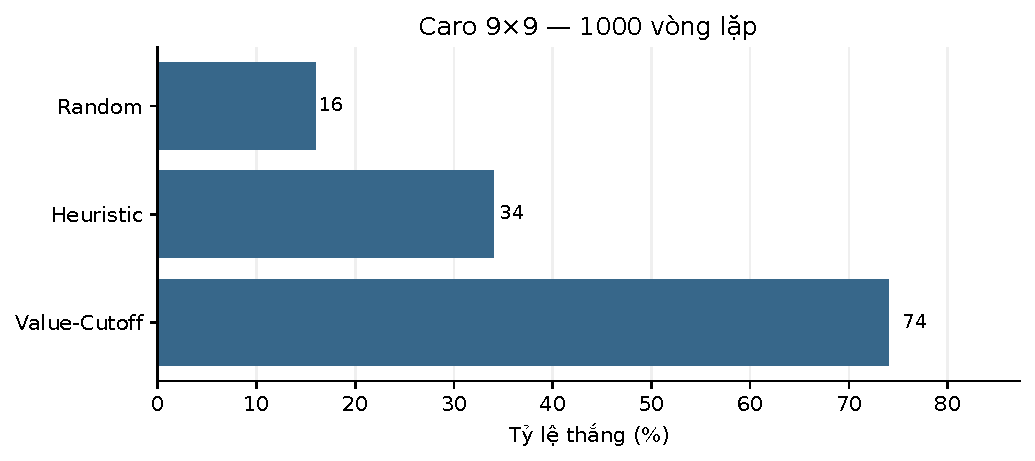
\includegraphics[width=.49\linewidth]{figures/03_rollout_win.pdf}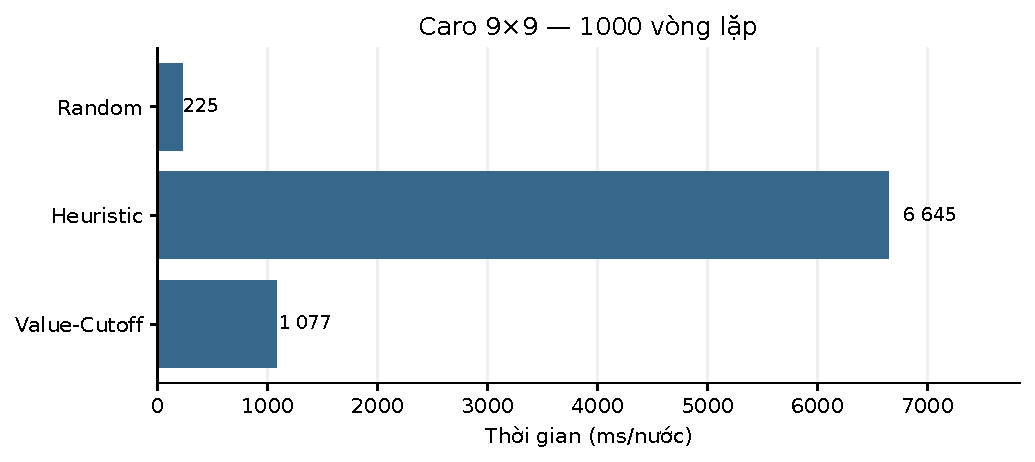
\includegraphics[width=.49\linewidth]{figures/04_rollout_time.pdf}\caption{Minh họa lại kết quả tại 1000 vòng lặp trong Hình 3 gốc.}\end{figure}
Trong thí nghiệm bảy biến thể (500 vòng), bỏ căn bậc hai làm tỷ lệ thắng giảm xuống 16\%. UCB1-Tuned nâng UCT tiêu chuẩn từ 28\% lên 42\%; PUCT đạt 98\% (49 thắng, 1 hòa, 0 thua).
\fig{05_uct}{.90}{Đánh giá các thành phần và cải tiến công thức UCT (Hình 4 gốc).}
\subsection{Mở rộng: Cờ tướng và định tuyến giao hàng}
\begin{table}[H]\centering\caption{Kết quả mở rộng trên Cờ tướng và TSP-TW}\small
\begin{tabular}{lrrr}\toprule Thuật toán và đối thủ & Thắng & Thắng/Hòa/Thua & ms\\\midrule
AB ($d=2$) vs Random&88\%&44/6/0&47,1\\
MCTS-ValueCut vs Random&96\%&48/0/2&206,1\\
PUCT-ValueCut vs Greedy&90\%&45/5/0&185,6\\\bottomrule\end{tabular}\par\medskip
\begin{tabular}{llrl}\toprule Quy mô & Thuật toán & Chi phí & Sai lệch / so sánh\\\midrule
8 & Nearest Neighbor &480,1&126,7\%\\
8 & EDF &679,4&198,6\%\\
8 & MCTS-Heuristic &248,7&4,78\%\\
8 & Exact BnB &235,3&0,00\%\\
16 & Nearest Neighbor &2548,7&Mốc so sánh\\
16 & EDF &3592,1&Mốc so sánh\\
16 & MCTS-Heuristic (1500 vòng)&1436,8&Giảm 43,6\% so với NN\\\bottomrule\end{tabular}\end{table}
Thời gian báo cáo: 0,1 ms cho cặp NN/EDF, 57,6 ms cho nhóm MCTS-Heuristic/Exact BnB ở 8 đơn và 185,2 ms cho MCTS-Heuristic ở 16 đơn. NN chọn điểm gần nhất; EDF ưu tiên hạn sớm nhất; BnB là nhánh cận.
\fig{06_xiangqi}{.90}{Tỷ lệ thắng trên Cờ tướng qua 50 ván (minh họa Hình 5a gốc).}
\fig{07_delivery}{.85}{Chi phí định tuyến với 16 đơn (minh họa một phần Hình 5b gốc).}
\section{Thảo luận}
\subsection{Vì sao max N tốt hơn max W/N?}
Nước đi có mẫu nhỏ ($N=1$–$2$) có thể đạt 100\% thắng chỉ do may mắn, với sai số chuẩn lớn ($\sim0.5/\sqrt N$). Số lượt truy cập phản ánh khả năng duy trì hiệu quả trước phản kháng trong UCT: nước đi được truy cập 795 lần đã vượt qua hàng trăm lần tìm kiếm phản bác của đối thủ.
\subsection{Tiền thân của mạng giá trị và mạng chính sách}
Thay mô phỏng toàn ván nhiều nhiễu bằng Value-Cutoff sau bốn lượt đi nâng tỷ lệ thắng Caro từ 16\% lên 74\% và Cờ tướng trước Random từ 66\% lên 96\%, nhanh hơn 8,4 lần. PUCT có tiên nghiệm heuristic đạt 98\%. Thay các bộ ước lượng thủ công bằng mạng neural sâu Value và Policy là bước đột phá của AlphaGo Zero và AlphaZero [6,7].
\subsection{Hạn chế}
Python thuần giới hạn độ sâu Alpha–Beta và tốc độ MCTS so với C++. Bán kính ứng viên Caro $r=2$ là thu hẹp heuristic. Cờ tướng chưa triển khai quy định liên đoàn châu Á về đuổi quân liên tục.
\section{Kết luận}
Nghiên cứu kiểm chứng Minimax + Alpha–Beta và MCTS–UCT trên Tic-Tac-Toe 3×3, Caro 5 quân, Cờ tướng 9×10 và lập lịch giao hàng thực tế. Hoeffding giải thích cấu trúc căn bậc hai và logarithm của UCT. Các thí nghiệm cho thấy mức giảm nút tới 99,61\%, tỷ lệ thua 0\% trên Tic-Tac-Toe, vai trò điều chỉnh $c$ trong ngân sách hữu hạn, cải thiện từ UCB1-Tuned/PUCT và Value-Cutoff, cùng mức giảm chi phí 43,6\% trong logistics chặng cuối.
\section*{Tài liệu tham khảo}
\small
[1] C. E. Shannon, “Programming a computer for playing chess,” \textit{Phil. Mag.}, 41(314), 256–275, 1950.

[2] D. E. Knuth và R. W. Moore, “An analysis of alpha-beta pruning,” \textit{Artificial Intelligence}, 6(4), 293–326, 1975.

[3] P. Auer, N. Cesa-Bianchi và P. Fischer, “Finite-time analysis of the multiarmed bandit problem,” \textit{Machine Learning}, 47, 235–256, 2002.

[4] L. Kocsis và C. Szepesvári, “Bandit based Monte-Carlo planning,” Proc. ECML, Springer, 282–293, 2006.

[5] C. B. Browne và cộng sự, “A survey of Monte Carlo tree search methods,” \textit{IEEE Trans. Comput. Intell. AI Games}, 4(1), 1–43, 2012.

[6] D. Silver và cộng sự, “Mastering the game of Go with deep neural networks and tree search,” \textit{Nature}, 529, 484–489, 2016.

[7] D. Silver và cộng sự, “Mastering the game of Go without human knowledge,” \textit{Nature}, 550, 354–359, 2017.

[8] S. Russell và P. Norvig, \textit{Artificial Intelligence: A Modern Approach}, ấn bản 4, Pearson, 2021.

\medskip\noindent\textit{Ghi chú bản dịch: Giữ nguyên số liệu và lập luận được báo cáo, chưa kiểm chứng độc lập. Biểu đồ được dựng lại theo số liệu đã nêu trong câu trả lời, không nội suy các điểm chưa có số liệu chính xác. Bố cục một cột để dễ đọc và chỉnh sửa.}
\end{document}
